\documentclass{article}
\usepackage{amssymb}
\usepackage{pdfpages}
\usepackage{hyperref}
\usepackage{cleveref}
\usepackage{enumitem}
\usepackage{graphicx} 
% set the margin of the document
\usepackage[a4paper, total={7in, 10in}]{geometry}

\newlist{todolist}{itemize}{2}
\setlist[todolist]{label=$\square$}
\newcommand{\cmark}{$\checkmark$}%
% \newcommanc{\xmark}{\ding{55}}%
\newcommand{\done}{\rlap{$\square$}{\raisebox{2pt}{\large\hspace{1pt}\cmark}}%
% \newcommand{\wontfix}{\rlap{$\square$}{\large\hspace{1pt}\xmark}}\hspace{-2.5pt}}
\newcommand{\notdone}{\rlap{$\square$}{\large\hspace{1pt}\xmark}}\hspace{-2.5pt}}



\hypersetup{
  colorlinks=true,
  allcolors=blue,
}

\renewcommand{\thesubsection}{\thesection.\Alph{subsection}}
    \title{
CS446 Deliverable 1 - Project Proposal \\
    Project Title: Pitch-Perfectly-Accurately Practice}
    \author{Irvine Yao (b6yao), Jialin Shan (j6shan), Alex Lai \ (x7lai), Johnny Gao (z53gao)}

\begin{document}
\maketitle

% set global enumerate line space
\setlist[enumerate]{topsep=0pt,itemsep=-1ex,partopsep=1ex,parsep=1ex}.
% set global itemize line space
\setitemize{noitemsep,topsep=0pt,parsep=0pt,partopsep=0pt}
\begin{center}
(Demo Youtube Video: \url{https://youtu.be/JqUM81U_XtY})
\end{center}
\section{Proposed Functionality From D1 and pivot}
\begin{todolist}
\item [\done] General UI 
\item [\done] Real time interaction with user’s voice
\item [\done] Jumping arrows
\item [\done] Note Practice Mode
\item [\done] Interval Practice Mode
\item [\done] Chord Practice Mode ( $\to$ Triad Practice Mode)
\item [\done] Song Practice Mode 
\item [$\ldots$] Song Mode Library to select songs ( $\to$ A temporary Spinner)
\item [\done] Filter Pages ( $\to$ per mode setting )
\item [\done] Note Summary Analysis
\item [\done] Left Menu ( $\to$ Navigation Menu )
\item [$\ldots$] Double tap to go to next question ( $\to$ Temporarily long press help button to go to next question )
\item [\done] PlaySound Button behaves according to the mode
\item [$\square$] Pages in “More” Menu 
\item [$\square$] Global settings (theme, etc..)
\item [x] Metronome (dropped)
\item [\done] Help Popup
\item [\done] First Launch tutorial 
\item [$\ldots$] Summary page (A mock version)
\item [\done] Real-time graph  (\textbf{Pivot})
\end{todolist}

\subsection{Current progress and future plan}
\begin{itemize}
  \item 
 Reasons for functionality in D1 to change/be dropped/not finished 
\begin{itemize}
  \item The chord mode is simplified to triad mode. 
    \begin{itemize}
      \item 
        Triad (has 3 notes) is a subset of chord mode (can have more than 3 notes). 
      \item 
        Chord mode can be added in the future. 
      \item 
        other priorities came first
    \end{itemize}
  \item 
    Missing song mode library
    \begin{itemize}
      \item 
        Will have in the future, currently using a spinner to select songs
    \end{itemize}
  \item 
    Per mode settings and global settings unfinished 
    \begin{itemize}
      \item 
        Currently only has a note / interval filter 
      \item 
        More settings in per mode hasn’t been implemented 
      \item 
        other priorities came first
    \end{itemize}
  \item
    Missing various Pages in More Menu, songlibrary, Double tap to next question
    \begin{itemize}
      \item 
        Reason: other priorities came first
    \end{itemize}
  \item
    Metronome dropped
    \begin{itemize}
      \item 
        For song playing mode, a metronome is annoying.
      \item 
        For song practice mode, user sings a note perfectly then next note, a metronome is not needed.
    \end{itemize}
\end{itemize}
\item{ Functionality planned (extended as ideas become concrete) but not proposed in D1 }

\begin{itemize}
  \item 
    Settings storage (can reload settings after kill and launch).
  \item
    Users can add their own midi and practice song.
\end{itemize}
\end{itemize}

\section{ Demo Summary and Plan  } 
    Note Mode $\to$ Graph Mode $\to$ Interval Mode $\to$ Triad Mode $\to$ Song Mode $\to$ Per Mode Settings 

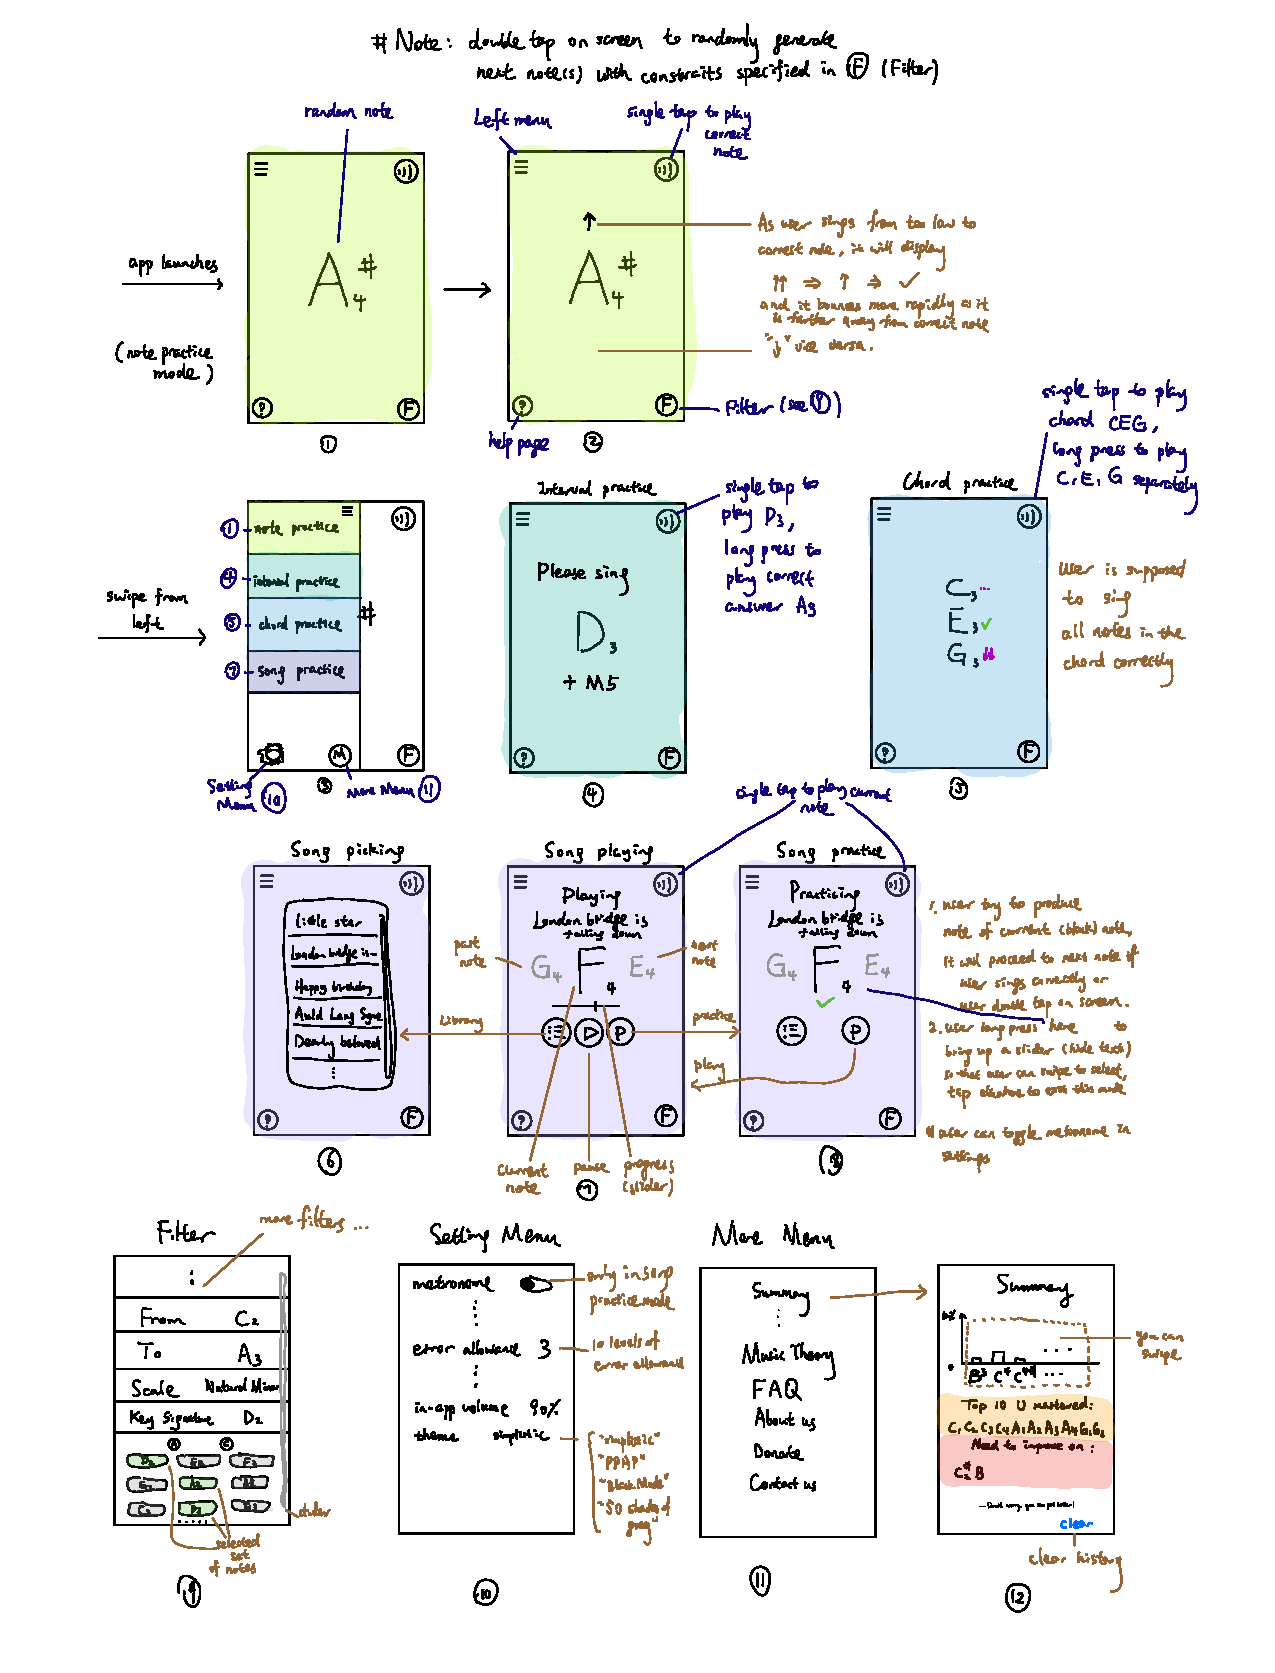
\includegraphics[page=1,width=.6\textwidth] {wireframes.pdf} Figure is Wireframe from D1

\end{document}
